\documentclass[serif]{beamer}\usepackage[]{graphicx}\usepackage[]{color}
%% maxwidth is the original width if it is less than linewidth
%% otherwise use linewidth (to make sure the graphics do not exceed the margin)
\makeatletter
\def\maxwidth{ %
  \ifdim\Gin@nat@width>\linewidth
    \linewidth
  \else
    \Gin@nat@width
  \fi
}
\makeatother

\definecolor{fgcolor}{rgb}{0.345, 0.345, 0.345}
\newcommand{\hlnum}[1]{\textcolor[rgb]{0.686,0.059,0.569}{#1}}%
\newcommand{\hlstr}[1]{\textcolor[rgb]{0.192,0.494,0.8}{#1}}%
\newcommand{\hlcom}[1]{\textcolor[rgb]{0.678,0.584,0.686}{\textit{#1}}}%
\newcommand{\hlopt}[1]{\textcolor[rgb]{0,0,0}{#1}}%
\newcommand{\hlstd}[1]{\textcolor[rgb]{0.345,0.345,0.345}{#1}}%
\newcommand{\hlkwa}[1]{\textcolor[rgb]{0.161,0.373,0.58}{\textbf{#1}}}%
\newcommand{\hlkwb}[1]{\textcolor[rgb]{0.69,0.353,0.396}{#1}}%
\newcommand{\hlkwc}[1]{\textcolor[rgb]{0.333,0.667,0.333}{#1}}%
\newcommand{\hlkwd}[1]{\textcolor[rgb]{0.737,0.353,0.396}{\textbf{#1}}}%

\usepackage{framed}
\makeatletter
\newenvironment{kframe}{%
 \def\at@end@of@kframe{}%
 \ifinner\ifhmode%
  \def\at@end@of@kframe{\end{minipage}}%
  \begin{minipage}{\columnwidth}%
 \fi\fi%
 \def\FrameCommand##1{\hskip\@totalleftmargin \hskip-\fboxsep
 \colorbox{shadecolor}{##1}\hskip-\fboxsep
     % There is no \\@totalrightmargin, so:
     \hskip-\linewidth \hskip-\@totalleftmargin \hskip\columnwidth}%
 \MakeFramed {\advance\hsize-\width
   \@totalleftmargin\z@ \linewidth\hsize
   \@setminipage}}%
 {\par\unskip\endMakeFramed%
 \at@end@of@kframe}
\makeatother

\definecolor{shadecolor}{rgb}{.97, .97, .97}
\definecolor{messagecolor}{rgb}{0, 0, 0}
\definecolor{warningcolor}{rgb}{1, 0, 1}
\definecolor{errorcolor}{rgb}{1, 0, 0}
\newenvironment{knitrout}{}{} % an empty environment to be redefined in TeX

\usepackage{alltt}
\usetheme{EPA}
\usepackage{graphicx}
\usepackage{xcolor}
\usepackage{tikz}
\usetikzlibrary{shadows,arrows,positioning,trees}

\newcommand{\emtxt}[1]{\textbf{\textit{#1}}}

\tikzstyle{block} = [rectangle, draw, text width=7em, text centered, rounded corners, minimum height=3em, minimum width=7em, top color = white, bottom color=brown!30,  drop shadow]

% knitr setup


\IfFileExists{upquote.sty}{\usepackage{upquote}}{}
\begin{document}

\title[NERRS Analysis Tools]{{\bf Five minutes in an elevator at 30000 feet over a mile-wide canyon}}

\author[M. Beck]{Marcus W. Beck}

\date{July 27, 2016}

\institute[]{\inst{1} USEPA NHEERL Gulf Ecology Division\\ Email: \href{mailto:beck.marcus@epa.gov}{beck.marcus@epa.gov}}

%%%%%%
\begin{frame}
\vspace{-0.1in}
\titlepage
\end{frame}

%%%%%%
\begin{frame}{Choosing your own adventure}
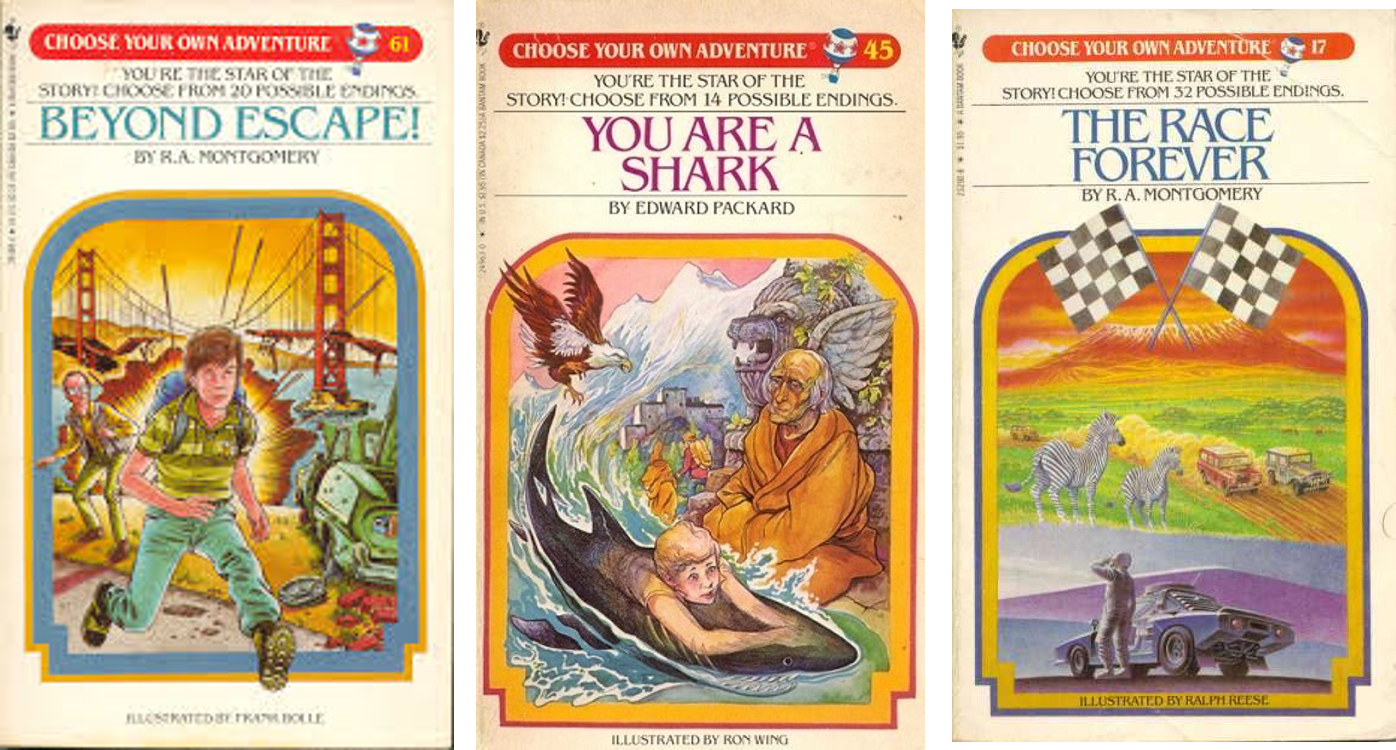
\includegraphics[width = \textwidth]{fig/Picture1.png}
\end{frame}

%%%%%%
\begin{frame}{Choosing your own adventure}
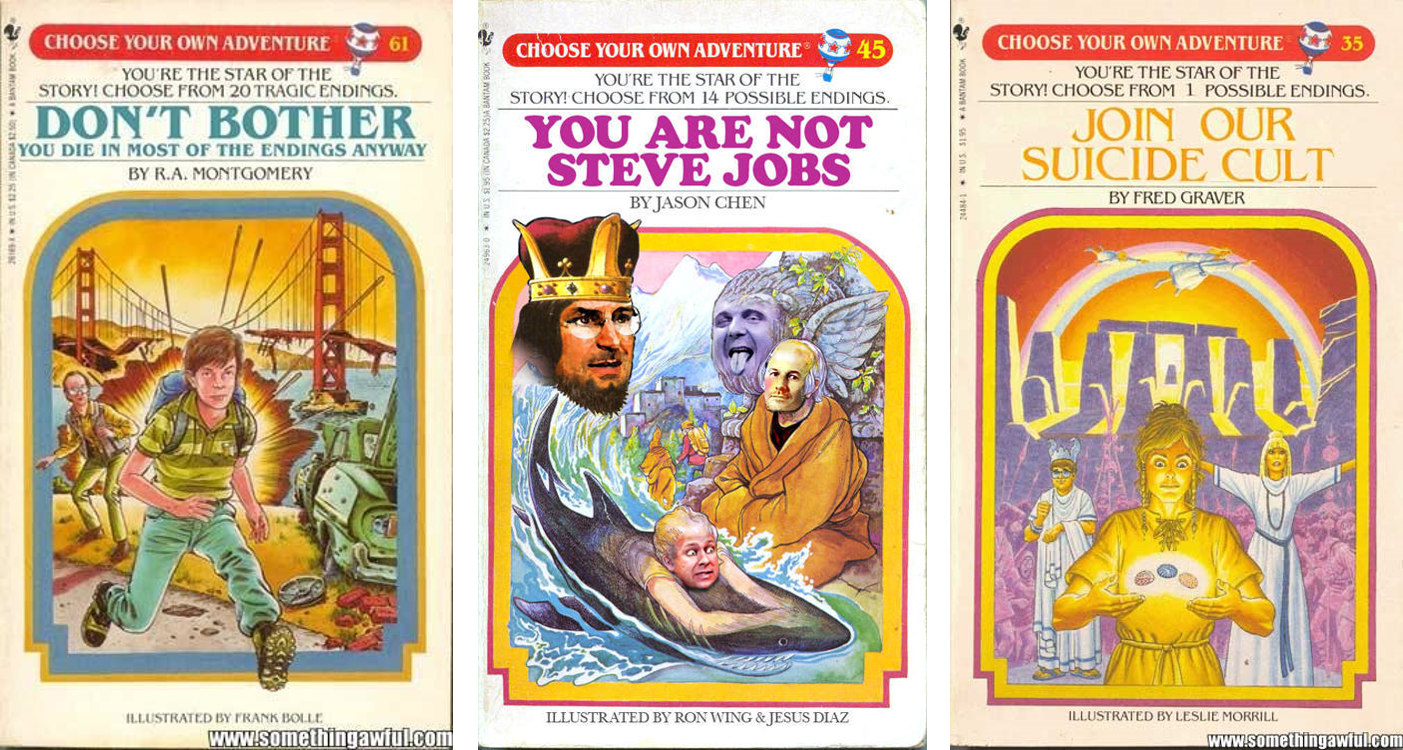
\includegraphics[width = \textwidth]{fig/Picture2.png}
\end{frame}

%%%%%%
\begin{frame}{Choosing your own adventure}
\setbeamercovered{again covered={\opaqueness<1->{45}}}
\begin{columns}[t]
\begin{column}{0.35\textwidth}
\onslide<1>
\underline{\textbf{13 years old}}\\~\\
\begin{enumerate}
\item Learn to fly \\~\\
\item Join Air Force \\~\\
\item Fighter pilot/ professional skateboarder
\end{enumerate}
\end{column}
\begin{column}{0.35\textwidth}
\onslide<2>
\underline{\textbf{20 years old}}\\~\\
\begin{enumerate}
\item BSc in Zoology \\~\\
\item Intern for FWC \\~\\
\item MSc in Conservation Biology \\~\\
\item Fisheries Biologist
\end{enumerate}
\end{column}
\begin{column}{0.35\textwidth}
\onslide<3>
\underline{\textbf{30 years old}}\\~\\
\begin{enumerate}
\setcounter{enumi}{3}
\item Intern for MNDNR \\~\\
\item PhD in Conservation Biology \\~\\
\item ORISE post-doc \\~\\
\item Fed post-doc \\~\\
\end{enumerate}
\end{column}
\end{columns}
\onslide<3>
\begin{tikzpicture}[overlay]
\draw[thick,->] (6.7,2.8) -- (7.9,4.75);
\end{tikzpicture}
\end{frame}

%%%%%%
\begin{frame}[t]{Elements of the adventure}

% \setbeamercovered{again covered={\opaqueness<1->{45}}}
\begin{columns}[T]
\begin{column}{0.5\textwidth}
  \begin{itemize}
  \setlength\itemsep{1.5em}
    \only<1>{ 
      \item Water quality
      \item Biological monitoring
      \item Eutrophication
      \item Aquatic Macrophytes
      \item Ecosystem metabolism
    }
    \only<2>{
      \item NeuralNetTools
      \item SWMPr
      \item WtRegDO
      \item WRTDStidal
      \item ggord
      \item rStrava
    }
    \only<3->{
      \item Indicator development
      \item Time series methods
      \item Reproducible research
      \item Visualization and graphics
      \item Model comparisons
    }
  \end{itemize}
\end{column}

\begin{column}{0.4\textwidth}
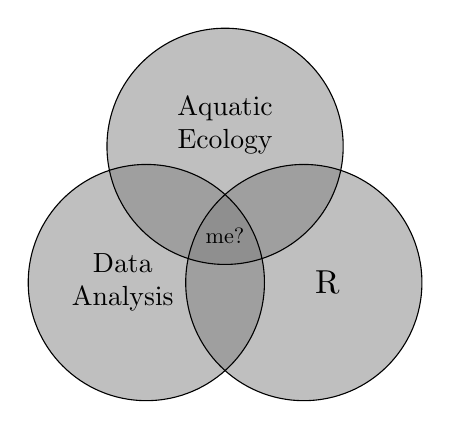
\begin{tikzpicture}
  \begin{scope}

    % The transparency:
    \begin{scope}[fill opacity=0.5]
      \onslide<3->\fill[gray] (-1, 0) circle (1.5);
      \onslide<2->\fill[gray] (1, 0) circle (1.5);
      \onslide<1->\fill[gray] (0, 1.73) circle (1.5);
    \end{scope}
    
    % letterings and missing pieces:
    \onslide<3->\draw[align=center] (-1, 0) circle (1.5);
    \onslide<2->\draw[align=center] (1, 0) circle (1.5);
    \onslide<1->\draw[align=center] (0, 1.73) circle (1.5);
    \onslide<3->\draw (-1.3, 0) node[scale=1,align=center] {Data \\ Analysis};
    \onslide<2->\draw (1.3, 0) node[scale=1.2] {R};
    \onslide<1->\draw (0, 2) node[scale=1,align=center] {Aquatic \\ Ecology};
 		\onslide<4->\draw (0, 0.6) node[scale=0.8] {me?};
 		
  \end{scope}
\end{tikzpicture}
\end{column}
\end{columns}
\end{frame}

% %%%%%%
% \begin{frame}[t]{Elements of the adventure}
% \onslide<1->
% \centerline{
\includegraphics[width = 0.8\textwidth]{fig/lopaper.png}} 
% \vspace{0.1in}
% \begin{columns}[T]
%   \begin{column}{0.3\textwidth}
%    \onslide<1->
%     \textbf{\underline{Ecology}}\\~\\
%     Can we get `better' metabolic estimates?
%   \end{column}
%   \begin{column}{0.3\textwidth}
%     \onslide<2->
%     \textbf{\underline{R}}\\~\\
%     \texttt{WtRegDO} software package as supplement
%   \end{column}
%   \begin{column}{0.3\textwidth}
%     \onslide<3->
%     \textbf{\underline{Data analysis}}\\~\\
%     Novel application of WRTDS method and online viz products
%   \end{column}
% \end{columns}
% \end{frame}

\end{document}
